\documentclass[11pt]{article}
\usepackage[margin=2.5cm]{geometry}
\usepackage[T1]{fontenc}
\usepackage{lmodern}
\usepackage{graphicx}
\usepackage{booktabs}
\usepackage{amsmath}
\usepackage[numbers,sort&compress]{natbib}
\usepackage[hidelinks]{hyperref}
\usepackage{setspace}
\onehalfspacing

\title{Adjustment and external replication of drug--hearing-loss signals:
a disproportionality analysis of FAERS and Canada Vigilance}
\author{Oleg Tropynin\\ \small Independent researcher, Karaganda, Kazakhstan\\ \small \texttt{tropininoleg@gmail.com}
\quad ORCID: \href{https://orcid.org/0009-0006-5431-4285}{0009-0006-5431-4285}}
\date{}

\begin{document}
\maketitle

\begin{abstract}
\noindent\textbf{Introduction:} Recent analyses of the US Food and Drug Administration Adverse Event
Reporting System (FAERS) reported many drug--hearing-loss signals absent from labels. We assessed which survive adjustment for
hearing-specific biases and external replication.

\noindent\textbf{Methods:} Disproportionality analysis of 19.9 million deduplicated FAERS reports
(2004--2026) and 1.2 million Canada Vigilance reports, following a protocol committed before
analysis. For hearing loss and tinnitus, crude reporting odds ratios (signal: lower 95\% bound $>1$, $\geq$3 cases) were
compared with Mantel--Haenszel estimates stratified by age, sex and period after excluding ear-related indications, reports
naming established ototoxic drugs and lawyer reports. Methods were compared on a label-derived reference set (area under the
receiver operating characteristic curve, AUC) and by replication in Canada Vigilance; robust unlabelled signals underwent
case-by-case review.

\noindent\textbf{Results:} Adjustment substantially changed the hearing-loss signal list
(63 of 300 crude signals lost, 73 gained) but not agreement
with labels (AUC, crude vs adjusted lower bound: 0.718 vs
0.723). Unlabelled signals replicated in Canada more than background but less than labelled ones; power-calibrated (post hoc), labelled signals replicated as predicted (observed/expected
1.02, 95\% CI 0.77--1.32)
and unlabelled ones did not (0.44, 0.29--0.62),
also within strata of consumer reporting. Solicited reports, report clusters and shared
co-medication produced spurious replications. Of 22 robust unlabelled signals (post hoc), 15 had artefactual or known
explanations; 7 remained (2--9 under
alternative choices).

\noindent\textbf{Conclusions:} Most unlabelled FAERS hearing-loss signals do not survive adjusted replication and provenance
review. Findings are hypothesis-generating; cross-database replication needs adjusted estimates and explicit
handling of solicited reports.
\end{abstract}

\section*{Key points}
\begin{itemize}
\item Adjusting FAERS hearing-loss screens for indication, ototoxic co-medication and stimulated reporting changes which drugs
are flagged but not their agreement with drug labels.
\item In Canada Vigilance, labelled hearing-loss signals replicated about as often as predicted and unlabelled ones less than half
as often, also among drugs with similar consumer reporting; solicited reports and shared co-medication produced spurious
replications.
\item After adjusted replication and case-by-case review of report provenance, 7 of 22 robust unlabelled signals
remained; they are hypotheses for exposure-based studies, not established adverse effects.
\end{itemize}

\section{Introduction}
The classical ototoxic drugs---aminoglycosides, platinum agents, loop diuretics, quinine, salicylates---were identified
mainly through clinical observation and case series \cite{lanvers2017}. For newer drugs, spontaneous reports are often the
first evidence, and recent studies have screened the FDA Adverse Event Reporting System (FAERS) across all drugs for
hearing-loss signals \cite{li2024,wu2025,liu2025} and for tinnitus \cite{narasimhaswamy2026,wang2024}, as have national
databases in Japan and France \cite{tanaka2019,favreliere2020}. These screens identify many unlabelled signals, but few
evaluate whether those signals survive adjustment and independent replication.

The FAERS screens share a design: crude disproportionality across all reports, with novelty defined as absence from the
label. This design is open to biases specific to hearing outcomes. Corticosteroids, vasodilators and antivirals are
prescribed \emph{for} sudden hearing loss and tinnitus, and several diseases cause hearing loss themselves (confounding by
indication). A drug routinely given with a strongly ototoxic one---an antiemetic with cisplatin, an antibiotic with an
aminoglycoside---inherits part of the association (co-medication bias). Reporting can be stimulated by safety
communications, litigation or media attention \cite{pariente2007}. Editorials have questioned disproportionality analyses
that ignore such biases \cite{ramessur2025}, and signal lists are rarely tested against an independent data source or a
reference set, as is done in evaluations of signal-detection methods \cite{harpaz2013}.

We therefore asked a narrower question than ``which drugs are ototoxic?'': \emph{which hearing-loss and tinnitus signals
remain after adjustment for these biases, and do the signals that remain replicate in an independent national database
and over time?} We compared crude and adjusted detection against a reference set derived from US labels, replicated every
signal in Canada Vigilance, re-tested the signals reported by previous FAERS screens, and reviewed the report provenance
of every robust unlabelled signal.

\section{Methods}
The study is reported according to the READUS-PV guideline \cite{readuspv,readuspv_ee}; the checklist is given in
Supplementary Table~S1. Primary analysis decisions were committed before the first result was computed; all later analyses
are labelled post hoc. The protocol, with all definitions and thresholds of the primary analysis, was committed to a
version-controlled repository at 02:05 UTC+5 on 26 October 2026 (git commit ff77c40). The first disproportionality estimates
were produced at 02:47--02:49 the same night; before that, only data preparation, the label reference set and tests on
simulated data had been run. The repository is controlled by the author and the protocol was not registered with a third
party. Every later change is dated and labelled in the protocol file (\texttt{PROTOCOL.md}). Figure~\ref{fig:workflow}
separates the pre-specified analyses from those added after the primary results were seen.

\begin{figure}[!tbp]
\centering
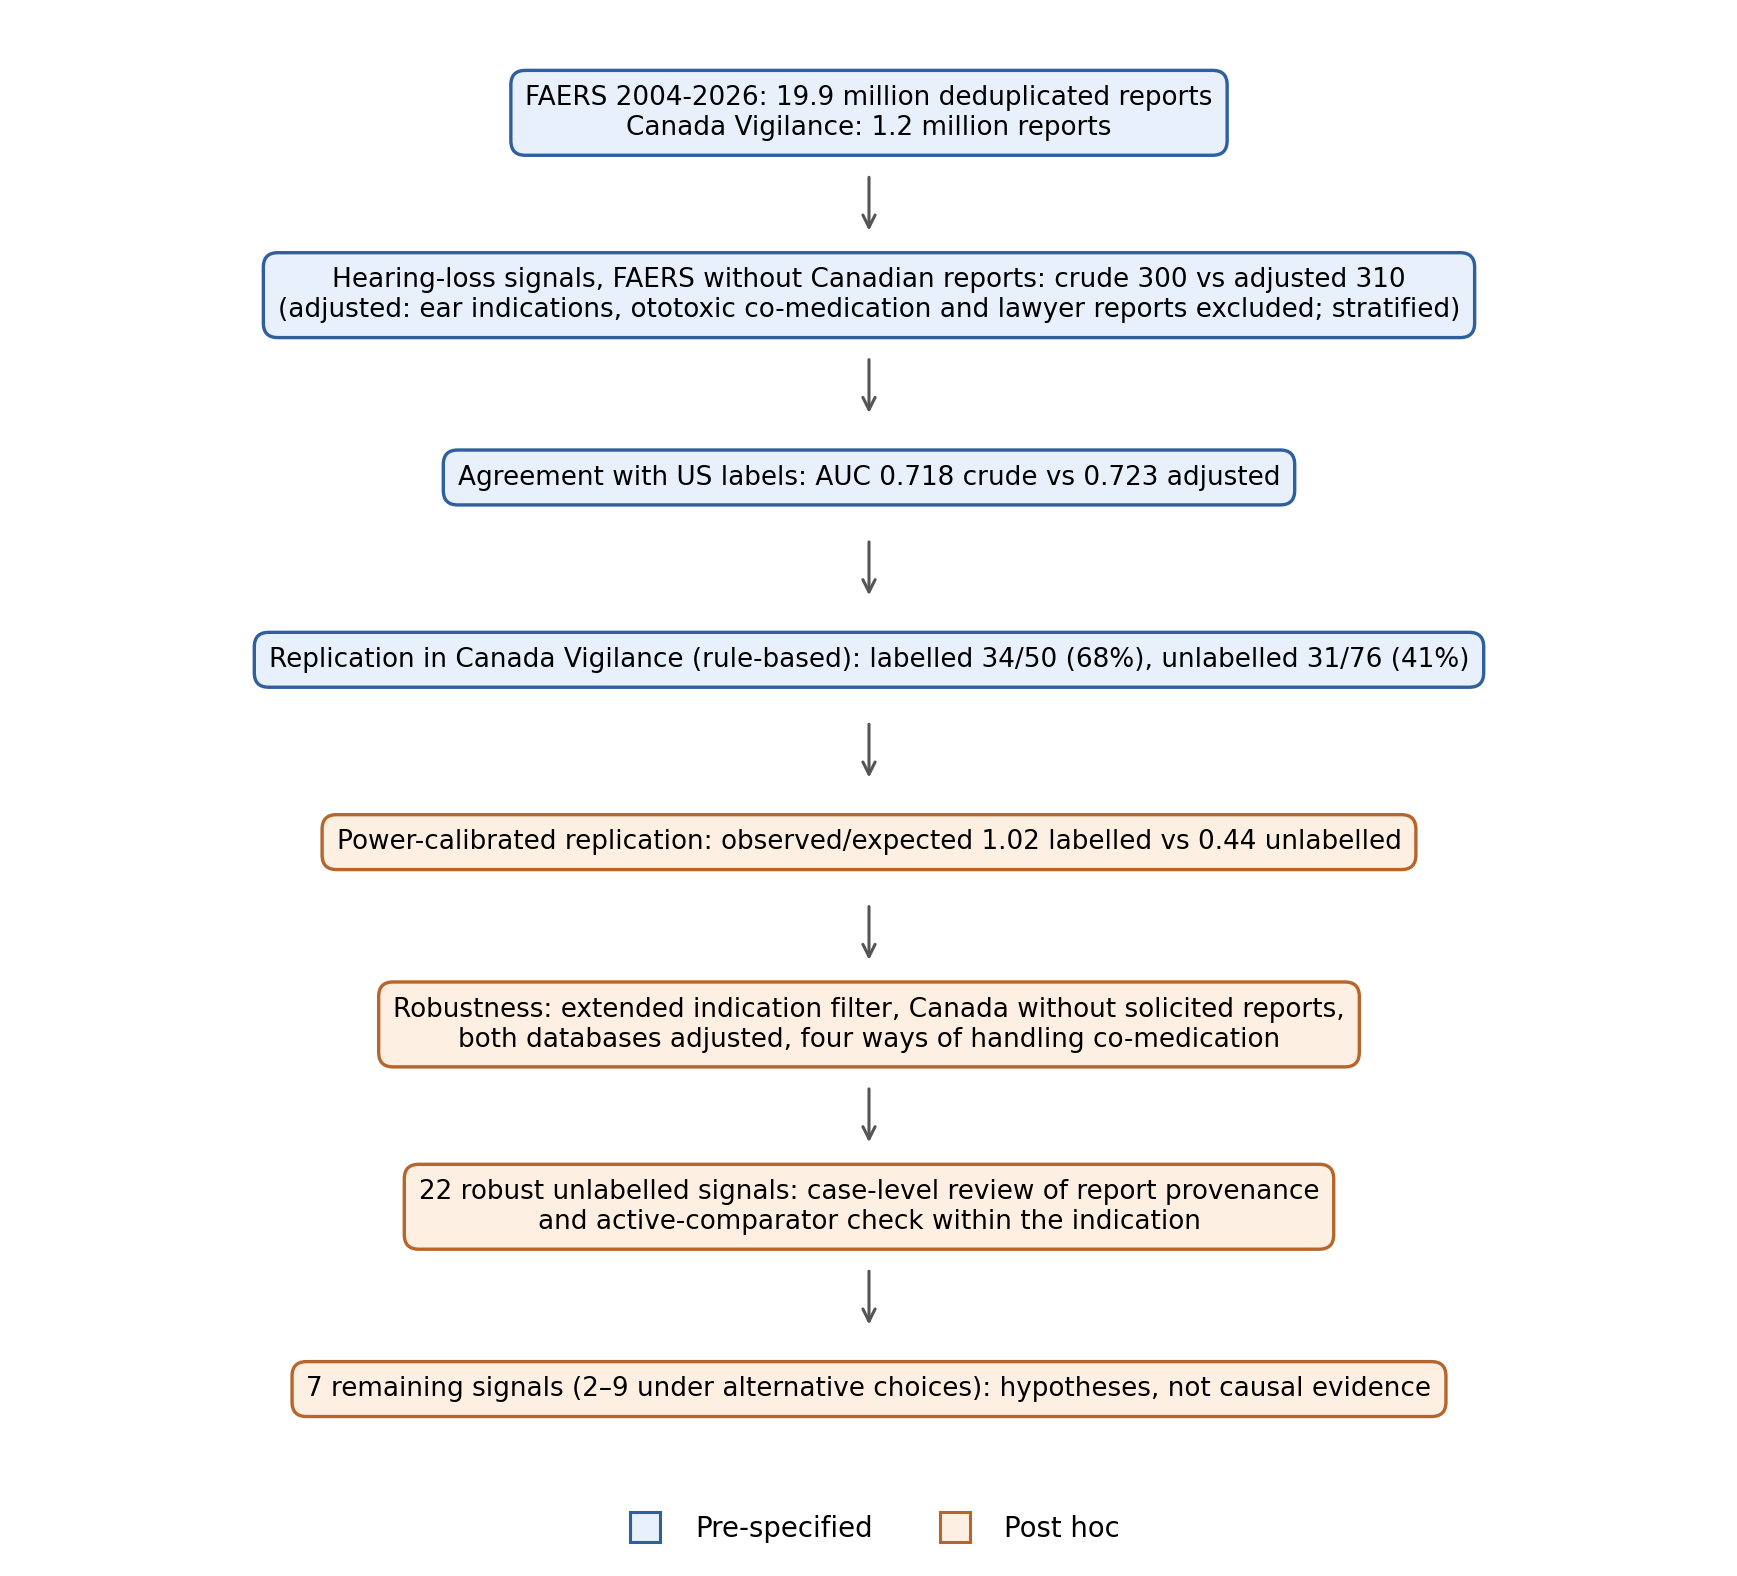
\includegraphics[width=0.72\textwidth]{../figures/workflow.png}
\caption{Study workflow. Blue: pre-specified analyses (protocol committed before the first result). Orange: analyses added
after the primary results were seen (post hoc). The remaining signals are hypotheses, not evidence of causation.}
\label{fig:workflow}
\end{figure}

\subsection{Data sources}
We used all 90 quarterly ASCII extracts of the legacy Adverse Event Reporting System (2004Q1--2012Q3) and FAERS
(2012Q4--2026Q2), published by the US Food and Drug Administration; the Canada Vigilance Adverse Reaction Online Database
extract (Health Canada; reports received 1965 to 30 June 2026); and the openFDA bulk export of structured product labels
(23 October 2026) \cite{openfda}. Events are coded in MedDRA preferred terms (PTs), at the version current when each
quarter was released (FAERS) and version 29.0 (Canada Vigilance); outcome terms were matched by preferred-term name, which
is stable across these versions for the terms used. All data are public and de-identified.

\subsection{Pre-processing and deduplication}
In FAERS we kept the most recent version of each case (by FDA receipt date, preferring FAERS over legacy records, then case
version), removed cases on FDA deletion lists, removed report identifiers recorded under two case numbers, and collapsed
content duplicates: reports with identical sex, age, event date, country, set of suspect ingredients and set of reactions
(applied only when event date and age were present). Drug names were mapped to active ingredients: the \texttt{prod\_ai}
field was split into ingredients; salt and hydrate words were removed when the remaining base was itself an observed
ingredient; free-text names in records without \texttt{prod\_ai} were mapped to the dominant ingredient recorded for that
name ($\geq$70\% of $\geq$5 records); INN/USAN synonyms were merged (for example glycopyrronium and glycopyrrolate);
four-letter biologic suffixes were removed; and non-specific entries (for example ``vitamins'', ``minerals'', ``\ldots{} NOS'')
were dropped. Combination products contribute to each of their ingredients. In Canada Vigilance, reports flagged as
duplicates of a report present in the extract were removed and product ingredients were normalised with the same rules.

\subsection{Outcomes, exposure and comparator}
The primary outcome, hearing loss, comprised the MedDRA PTs Deafness; Deafness unilateral, bilateral, neurosensory,
transitory, permanent and mixed; Hypoacusis; Neurosensory hypoacusis; Sudden hearing loss; Ototoxicity; Hearing impaired;
Hearing disability; and High frequency hearing loss. Conductive and congenital deafness were excluded. The secondary outcome
was Tinnitus. An ingredient was exposed when reported as a suspect drug (FAERS primary suspect, secondary suspect or
interacting; Canada suspect or interacting). The comparator for each ingredient was all other reports in the same
population. Missing age and sex formed their own strata; missing indication or country was treated as not meeting the
corresponding exclusion.

\subsection{Disproportionality}
For each ingredient we computed the reporting odds ratio (ROR) with a Woolf 95\% confidence interval \cite{woolf1955,rothman2004}
and the information component (IC) with its lower credibility bound IC$_{025}$ \cite{noren2006}. A \emph{crude signal}
required at least three cases, a lower ROR bound above 1 and IC$_{025}>0$.

The pre-specified \emph{adjusted} analysis was run in a restricted population and stratified. We excluded (i) reports in
which any drug had an ear or hearing indication (deafness, hearing, tinnitus, ototoxicity, M\'eni\`ere's disease, otitis,
vertigo, vestibular, labyrinthine and cochlear terms); (ii) reports that mentioned, in any role, a drug from an a-priori list
of 29 drugs from the established ototoxic classes \cite{lanvers2017} (aminoglycosides, capreomycin and vancomycin; cisplatin,
carboplatin and oxaliplatin; loop diuretics; quinine and related antimalarials; aspirin; macrolides; deferoxamine;
vincristine; eflornithine) other than the drug under study; and (iii) FAERS reports submitted by lawyers (Canada Vigilance
does not record this). For a drug on the list, reports naming the drug itself in a non-suspect role were also removed from
its population. We then computed the Mantel--Haenszel (MH) OR \cite{mantel1959} over 60 strata (five age bands $\times$ sex
[male, female, unknown] $\times$ four periods of report receipt: before 2004, 2004--2012, 2013--2018, 2019--2026) with the Robins--Breslow--Greenland variance \cite{robins1986}. An
\emph{adjusted signal} required at least three cases in the restricted population and a lower 95\% bound above 1. The
implementation reproduces \texttt{statsmodels} estimates on simulated data to nine decimal places.

\subsection{Reference set}
From single-ingredient US labels we classified each ingredient as label-positive when a hearing-loss term appeared in a
safety section (boxed warning, warnings, precautions, adverse reactions, post-marketing experience, contraindications,
overdosage, drug abuse and dependence, or the corresponding over-the-counter sections) of at least half of its prescription
labels, and label-negative when no label mentioned hearing loss or tinnitus; other ingredients were left out. Phrases that
contain a hearing word without describing an adverse effect (for example the disease name ``maternally inherited diabetes and
deafness'' and telephone lines for deaf users) were removed first. Discrimination was measured by the area under the ROC
curve (AUC) among ingredients with $\geq$1{,}000 suspect FAERS reports, comparing the crude and adjusted lower 95\% bounds
(the like-for-like pair; the protocol pre-specified the crude IC$_{025}$, which is also reported) and point estimates; the difference was bootstrapped (2{,}000
resamples). Because labels are partly informed by spontaneous reports, the reference set compares methods with each other;
it does not estimate absolute accuracy.

\subsection{Replication}
For external replication, signals were derived in FAERS after removing reports of Canadian origin and tested in Canada
Vigilance. Pre-specified rule: an ingredient was testable when the observed or expected number of Canadian cases was at
least three, and replicated when the Canadian lower ROR bound exceeded 1 with at least three cases. The same rule applied to
label-negative ingredients that were neither crude nor adjusted FAERS signals gave the background rate of replication
without a known association; label-negative ingredients that \emph{were} adjusted signals form a second reference group.
Because the testability rule depends on the observed count, we also computed a power-calibrated comparison (post hoc): for
every ingredient with a Canadian expected count $E>0$, replication was defined as an observed count of at least
$a_{\mathrm{crit}}$, the smallest count $\geq 3$ with Poisson $P(X\geq a\mid E)<0.025$, and the expected number of
replications was $\sum_i P(X\geq a_{\mathrm{crit},i}\mid E_i \times \mathrm{OR}_i)$, with OR$_i$ the adjusted FAERS
estimate shrunk towards the null by empirical Bayes (log OR $\times\,\tau^2/(\tau^2+\mathrm{se}^2)$, with $\tau^2$ estimated
across all ingredients) to counter the selection of signals on their estimate; observed-to-expected ratios near 1 indicate that
signals replicate as often as their FAERS strength predicts. Confidence intervals were bootstrapped over ingredients (2{,}000
resamples). In the post-hoc adjusted-to-adjusted analysis the Canadian adjusted case count was compared with its stratified
expected count. For
temporal replication, signals derived from reports received up to 2014 were tested in reports received from 2015 onwards.
Rates were compared with Fisher's exact test.

\subsection{Post-hoc and sensitivity analyses}
After the primary results were seen we added: Canada Vigilance without solicited reports (``Study'' report type, which
includes manufacturers' patient-support programmes); an extended indication filter (further ear terms; diseases that
themselves cause hearing loss, such as Fabry disease, mucopolysaccharidoses, cryopyrin-associated syndromes, meningitis,
giant cell arteritis and thyroid eye disease; and reports of prenatal exposure); and replication in which the Canadian
estimate is adjusted in the same way as the FAERS one (\emph{adjusted-to-adjusted}). In this post-hoc framework, ototoxic
co-medication was handled in three further ways: as a stratum dimension instead of an exclusion (because restricting on a
variable that reporters may add after observing hearing loss can introduce selection bias), with a short list of strongly
ototoxic drugs only, and after excluding reports that list 15 or more drugs (report clusters). Canada Vigilance was also
restricted to reports received from 2004.

\subsection{Robust signals and case-level review}
A \emph{robust signal} (post hoc) was an adjusted FAERS signal that replicated adjusted-to-adjusted in Canada Vigilance
without solicited reports. Throughout, a signal is \emph{labelled} when the event is mentioned in any safety section of any US label of a product
containing the drug (single-ingredient or combination) and \emph{unlabelled} otherwise, including drugs with no US label in the
export; \emph{label-positive} and \emph{label-negative} refer to the stricter reference-set classes. Robust unlabelled signals
were reviewed. For each we profiled the FAERS case series (without Canadian reports):
share of cases from the most frequent country and receipt year, consumer reports, reports listing $\geq$15 drugs, reports
co-naming an established ototoxic drug, prenatal exposure and leading indications; we searched PubMed for the drug with
hearing terms. Each signal was assigned the first applicable category of a written rubric: K, established ototoxic class or
association documented by a prospective or cohort clinical series; A, report cluster ($\geq$50\% of cases in reports listing
$\geq$15 drugs); B, ototoxic co-medication ($\geq$50\% of cases co-name an established ototoxic drug); C, stimulated or
solicited reporting documented for the drug; D, main indication itself associated with the event; E, none of these. The
rubric distinguishes C from D only on documented evidence; a high consumer share alone does not make a signal C. Because
confounding by indication remained plausible after the indication exclusions (reported indications are often missing or
non-specific), for category D we additionally required that the signal not persist against other drugs used for the same indication: within
FAERS reports (without Canadian origin) whose indication matched the drug's main indication, we computed the ROR of the drug
against all other suspect drugs (active-comparator check, post hoc). The author applied the rubric, and a second, AI-based
assessor applied it blind to the author's assignments, with the same profiles and literature access; agreement is reported as
Cohen's $\kappa$.

\subsection{Software and use of AI tools}
Analyses used Python 3.10 (numpy 2.2.6, pandas 2.3.3, scipy 1.15.3, statsmodels 0.15.0, matplotlib 3.10.9). An AI
assistant (Claude, Anthropic) wrote the code and the first draft of the manuscript under the author's direction, and AI
reviewers critiqued the methods, clinical interpretation and text; changes made in response are recorded in the protocol
file. The second assessor of the case-level review was also AI-based. The author reviewed the code, results and text and is
responsible for them.


\section{Results}

\subsection{Data}
The 90 FAERS extracts held 24{,}812{,}424 report versions, from which 20{,}692{,}682
cases remained after keeping the latest version; 104{,}186 cases on FDA deletion lists, cases without a
reaction or mappable ingredient, 1{,}681 report identifiers recorded under two cases and
510{,}312 content duplicates were then removed, leaving \textbf{19{,}876{,}330
reports} (4\% of drug rows could not be mapped; Supplementary Figure~S1). They contained
83{,}883 hearing-loss and 42{,}900 tinnitus reports; hearing-loss reports
came more often from consumers and from patients aged $\geq$65 years than other reports (Supplementary Table~S4). Without
Canadian reports, the population used for signal detection held 19{,}135{,}329 reports and 8{,}122 suspect
ingredients; its adjusted subset excluded 18{,}735 reports with an ear or hearing indication,
1{,}712{,}914 reports naming a listed ototoxic drug and 484{,}957 lawyer reports,
leaving 16{,}962{,}022 reports (67{,}913 hearing-loss cases). Canada Vigilance
contributed 1{,}210{,}857 reports after removing 58{,}623 duplicates
(4{,}000 hearing-loss and 3{,}284 tinnitus reports).

Drugs of the established ototoxic classes gave strong signals in both databases (Supplementary Table~S2), for example
amikacin (FAERS adjusted OR 12.7 (11.6--13.9)), gentamicin (11.4 (9.8--13.2)) and cisplatin (4.3 (4.0--4.6)); so did
the PDE5 inhibitors sildenafil (3.9 (3.7--4.2)) and tadalafil (4.2 (3.9--4.6)), whose labels carry hearing-loss
warnings, and teprotumumab (59.8 (55.4--64.5)). Some label-positive drugs did not signal: oxaliplatin (crude ROR
0.44) and vardenafil (6 cases); carboplatin was a
crude signal that fell below 1 after adjustment (1.96 to
0.82), as did vincristine's estimate, an example of the sensitivity that the
co-medication filter costs.

\subsection{Adjustment changes the signal list but not its agreement with labels}
In FAERS without Canadian reports the crude rule flagged 300 ingredients for hearing loss and the adjusted
rule 310; 63 crude signals were lost and 73 appeared
(Table~\ref{tab:methods}). Against the reference set (106 label-positive and 927 label-negative
ingredients with $\geq$1{,}000 suspect reports), discrimination was moderate and practically identical. For the
like-for-like pair, crude versus adjusted lower bound, the AUC was 0.718 vs
0.723 (difference 0.005, 95\% CI -0.023 to
0.030); for the pre-specified pair, crude IC$_{025}$ versus adjusted lower bound, it was
0.720 vs 0.723. Adjustment thus changed which drugs were flagged
but brought almost no improvement in agreement with labels. The same held for point estimates (0.700 vs
0.705), after excluding the 83 ingredients without an estimable
adjusted bound (0.698 vs
0.703), at lower report thresholds, without the 29 listed
drugs, and for tinnitus (0.775 vs 0.777). Adjustment lowered
sensitivity (0.40 to 0.35) with little change in specificity
(0.866 to 0.873).

\subsection{Replication in Canada Vigilance}
Under the pre-specified rule, adjusted hearing-loss signals already on a label replicated in 34/50 (68\%)
of testable cases and unlabelled adjusted signals in 31/76 (41\%) (Table~\ref{tab:methods}).
Label-negative adjusted signals replicated in 21/54 (39\%) and crude-only signals in
9/21 (43\%). The background---label-negative ingredients that were neither crude nor adjusted signals---replicated
in 43/214 (20\%) (all label-negative ingredients, as literally specified in the protocol:
68/281 (24\%)). In this pre-specified comparison unlabelled signals replicated more
often than the background (odds ratio 2.74, Fisher $p<0.001$) but less
often than labelled signals.

The power-calibrated comparison (post hoc) placed this contrast on a common scale (Figure~\ref{fig:repl}). Labelled signals
(n=70 ingredients) replicated about as often as their shrunken FAERS estimates predicted
(31 observed vs 30.5 expected; O/E 1.02, 95\% CI 0.77--1.32). Unlabelled signals (n=201) replicated less than half as often
(25 observed vs 56.8 expected; O/E 0.44, 95\% CI 0.29--0.62); the ratio of the two was 0.43
(95\% CI 0.26--0.66). The
label-negative signals, a subset of the unlabelled group, behaved alike (18 observed vs 37.5 expected; O/E 0.48, 95\% CI 0.27--0.72). Results were the
same with unshrunken estimates, with the pre-specified label definition, and for tinnitus (60 observed vs 63.2 expected; O/E 0.95, 95\% CI 0.79--1.14 for
labelled and 22 observed vs 46.4 expected; O/E 0.47, 95\% CI 0.29--0.66 for unlabelled signals).

Unlabelled signals were more often reported by consumers (median share of FAERS cases
58\% vs 39\% for labelled signals) and
more often from the United States (67\% vs 50\%), so
provenance could explain the contrast. It did not: among signals with a consumer share at or below the median, O/E was
1.01 for labelled and
0.57 (95\% CI
0.27--0.93) for
unlabelled signals, and above the median 1.04 and
0.36. Pooled across ingredients (random effects), the Canadian ROR
was 3.60 (2.47--5.26)
for labelled and 1.59 (1.28--1.96)
for unlabelled signals: as a group, unlabelled signals were attenuated rather than absent.

The replication test was not conservative: label-negative non-signals replicated 4.2 times as often as expected without any association
(36 vs 8.5). Solicited reports explained much of this:
\emph{Study} reports, which include manufacturers' patient-support programmes, made up 61\%
of Canadian hearing-loss cases for the background drugs that replicated, against 14\% for
replicated labelled signals and 36\% overall; for ocrelizumab, mepolizumab and omalizumab the share
was 93\%, 93\% and 86\%, against
1\% for gentamicin and 1\% for cisplatin. The mirror image appeared in FAERS:
tafamidis (adjusted OR 4.3 (3.8--4.8)) had
361 hearing-loss reports in FAERS (86\% from consumers,
97\% from the United States) but none in Canada Vigilance against 3.4 expected, and
sacubitril (2{,}801 FAERS hearing-loss reports; 88\% from consumers) none against
1.9 expected (too few to be testable).

Co-medication bias can also replicate when crude estimates are compared. Etoposide, given in cisplatin-containing regimens,
was a crude signal in both databases (FAERS ROR 2.09 (1.91--2.28);
Canada 5.13 (3.68--7.14)); after adjustment the FAERS estimate reversed
(0.67 (0.46--0.98)) and the Canadian one rested on
2 cases (1.15 (0.29--4.64)). Temporal replication within FAERS
did not favour adjustment for hearing loss: early crude-only signals recurred after 2014 at least as often
(18/28 (64\%)) as early adjusted signals (81/155 (52\%); background 137/938 (15\%)),
consistent with biases that persist within one database; for tinnitus adjusted signals recurred more often
(100/121 (83\%) vs 9/15 (60\%)).

\subsection{Post-hoc analyses}
The post-hoc framework combined the extended indication filter, Canada Vigilance restricted to unsolicited reports and
adjusted estimates in both databases (Table~\ref{tab:posthoc}). In it, labelled hearing-loss signals replicated in
26/44 (59\%), unlabelled signals in 10/51 (20\%) and the background in 19/158 (12\%)
(Fisher $p=0.24$). Calibrated on adjusted Canadian counts, O/E was 1.10 (95\% CI
0.79--1.48) for labelled and
0.26 (0.11--0.43)
for unlabelled signals (ratio 0.24, 95\% CI
0.09--0.44); the pooled
Canadian adjusted OR was 4.25 (2.73--6.64)
for labelled, 1.37 (1.03--1.83)
for unlabelled and 1.29 (1.00--1.66)
for label-negative signals. For tinnitus, labelled signals replicated less fully in this framework (O/E
0.70, 95\% CI 0.54--0.88),
with unlabelled signals lower still (0.21). Across the co-medication variants and the restriction of Canada Vigilance to reports from 2004,
unlabelled O/E ranged 0.23--0.28 and labelled
0.94--1.18. The comparison with the background depended on
report clusters: after excluding reports that list $\geq$15 drugs, the background fell to 5/159 (3\%) and
unlabelled signals (8/48 (17\%)) exceeded it (Fisher $p=0.002$),
although still replicating far below expectation (O/E 0.27). Handling
co-medication as a stratum rather than an exclusion removed the below-1 estimates of label-positive drugs (carboplatin
0.79 to 1.34; vincristine
0.48 to 1.04), consistent
with selection bias from the exclusion, but did not remove the etoposide association
(1.57), consistent with residual co-medication bias under a binary stratum.

\subsection{Signals from previous screens}
Of the 23 hearing-loss signals that Li et al.\ classified as unlabelled \cite{li2024},
16 were crude and 16 adjusted signals in FAERS without Canadian reports,
6 were testable in Canada and 2 replicated; 1
met the post-hoc robust definition (glycopyrrolate). Their strongest unlabelled signals included
sacubitril/valsartan and tafamidis. Of the 28 unlabelled paediatric signals of Liu et al.\ \cite{liu2025},
11 were adjusted signals in our all-age data and 1 met the robust definition
(azithromycin, which is on the a-priori ototoxic list);
cefixime, ceftriaxone, etoposide and isoniazid were lost on adjustment (Table~\ref{tab:prior}). Only
abstract-level lists were available for the other screens (Supplementary Table~S6).

\subsection{Case-level review}
Under the post-hoc definition, 10 hearing-loss and 12 tinnitus signals were robust and absent from every US
label (Table~\ref{tab:cand}, Figure~\ref{fig:cand}). The review attributed 4 to report clusters (for
example candesartan--tinnitus: 80\%
of cases from the United Kingdom, median 42 drugs per
report), 6 to stimulated or mass-exposure reporting (mRNA COVID-19 vaccines, rofecoxib, finasteride),
1 to an established ototoxic class (oral paromomycin) and 4 to an indication, with an
active-comparator estimate consistent with it (etanercept against other rheumatoid-arthritis drugs,
ROR 0.93 (0.87--1.00); insulin aspart within diabetes, 1.17 (1.00--1.37); galcanezumab within migraine,
0.82 (0.63--1.06); and chlorthalidone within hypertension, 1.04 (0.43--2.51), which is indeterminate with
5 cases). For seven signals the
indication did not account for the association, because it persisted against other drugs for the same indication:
tofacitinib, pregabalin, amlodipine, glycopyrrolate and travoprost for hearing loss (for example pregabalin within pain and neuropathy, ROR 3.27 (3.04--3.52); amlodipine
within hypertension, 1.89 (1.69--2.10)) and doxycycline and liothyronine for tinnitus (doxycycline, 3.63 (2.98--4.42)).
A second, AI-based assessor applying the same rubric to the same profiles agreed on 19 of 22 assignments
before the active-comparator step (Cohen's $\kappa=0.82$) and on 19 after the same mechanical rule
was applied to both ($\kappa=0.82$); with its assignments, nine signals would remain unexplained
(Supplementary Table~S3). Before the post-hoc active-comparator rule, only two (pregabalin and doxycycline)
were unexplained; the residual count therefore ranges from 2 to 9 depending on post-hoc choices and assessor.

\begin{table}[t]
\centering\small
\caption{Crude versus adjusted detection (pre-specified analyses). Replication counts are replicated/testable ingredients.}
\label{tab:methods}
\begin{tabular}{p{8.6cm}cc}
\toprule
 & Crude & Adjusted \\
\midrule
\multicolumn{3}{l}{\textit{Hearing loss}} \\
Reference set, positive/negative ingredients & \multicolumn{2}{c}{106/927} \\
AUC, lower 95\% bound & 0.718 & 0.723 \\
\quad difference (95\% CI) & \multicolumn{2}{c}{0.005 (-0.023 to 0.030)} \\
Sensitivity / specificity of the signal rule & 0.40 / 0.87 & 0.35 / 0.87 \\
Signals (FAERS without Canadian reports) & 300 & 310 \\
Replicated in Canada$^a$: labelled adjusted signals & \multicolumn{2}{c}{34/50 (68\%)} \\
\quad unlabelled adjusted signals & \multicolumn{2}{c}{31/76 (41\%)} \\
\quad label-negative adjusted signals & \multicolumn{2}{c}{21/54 (39\%)} \\
\quad crude-only signals & \multicolumn{2}{c}{9/21 (43\%)} \\
\quad background (label-negative non-signals) & \multicolumn{2}{c}{43/214 (20\%)} \\
\quad all label-negative ingredients (protocol wording) & \multicolumn{2}{c}{68/281 (24\%)} \\
Observed/expected replications$^b$: labelled & \multicolumn{2}{c}{31/30.5 = 1.02 (0.77--1.32)} \\
\quad unlabelled & \multicolumn{2}{c}{25/56.8 = 0.44 (0.29--0.62)} \\
\quad label-negative & \multicolumn{2}{c}{18/37.5 = 0.48 (0.27--0.72)} \\
\midrule
\multicolumn{3}{l}{\textit{Tinnitus}} \\
Reference set, positive/negative ingredients & \multicolumn{2}{c}{186/927} \\
AUC, lower 95\% bound & 0.775 & 0.777 \\
\quad difference (95\% CI) & \multicolumn{2}{c}{0.002 (-0.016 to 0.018)} \\
Sensitivity / specificity of the signal rule & 0.51 / 0.85 & 0.50 / 0.87 \\
Signals (FAERS without Canadian reports) & 399 & 349 \\
Replicated in Canada$^a$: labelled adjusted signals & \multicolumn{2}{c}{65/89 (73\%)} \\
\quad unlabelled adjusted signals & \multicolumn{2}{c}{24/56 (43\%)} \\
\quad label-negative adjusted signals & \multicolumn{2}{c}{17/43 (40\%)} \\
\quad crude-only signals & \multicolumn{2}{c}{13/30 (43\%)} \\
\quad background (label-negative non-signals) & \multicolumn{2}{c}{31/193 (16\%)} \\
\quad all label-negative ingredients (protocol wording) & \multicolumn{2}{c}{53/252 (21\%)} \\
Observed/expected replications$^b$: labelled & \multicolumn{2}{c}{60/63.2 = 0.95 (0.79--1.14)} \\
\quad unlabelled & \multicolumn{2}{c}{22/46.4 = 0.47 (0.29--0.66)} \\
\quad label-negative & \multicolumn{2}{c}{16/33.8 = 0.47 (0.27--0.72)} \\
\bottomrule
\end{tabular}

\smallskip
\raggedright\footnotesize $^a$ Pre-specified rule: FAERS without Canadian reports; Canada crude ROR, all reports.
$^b$ Power-calibrated (post hoc): observed replications vs those expected if each FAERS adjusted estimate were true.
\end{table}

\begin{table}[t]
\centering\small
\caption{Post-hoc analyses: extended indication filter, Canada Vigilance without solicited reports, both estimates adjusted,
with four ways of handling ototoxic co-medication and a restriction of Canada Vigilance to reports from 2004. Fisher $p$:
unlabelled vs background replication. O/E: observed/expected replications (adjusted counts). Robust: adjusted signals replicated
adjusted-to-adjusted (unlabelled in brackets).}
\label{tab:posthoc}
\resizebox{\textwidth}{!}{%
\begin{tabular}{lcccccccc}
\toprule
Co-medication handling & Signals & AUC & Labelled repl. & Unlabelled repl. & Background repl. & Fisher $p$ & O/E lab./unlab. & Robust \\
\midrule
\multicolumn{9}{l}{\textit{Hearing loss}} \\
Exclusion (as primary) & 295 & 0.719 & 26/44 (59\%) & 10/51 (20\%) & 19/158 (12\%) & 0.242 & 1.10 / 0.26 & 36 (10) \\
Co-medication as stratum & 323 & 0.718 & 28/43 (65\%) & 17/57 (30\%) & 28/158 (18\%) & 0.060 & 0.94 / 0.25 & 45 (17) \\
Strong ototoxic list only & 303 & 0.714 & 26/43 (60\%) & 14/54 (26\%) & 22/158 (14\%) & 0.058 & 1.03 / 0.28 & 40 (14) \\
Without reports listing $\geq$15 drugs & 269 & 0.725 & 26/41 (63\%) & 8/48 (17\%) & 5/159 (3\%) & 0.002 & 1.18 / 0.27 & 34 (8) \\
Exclusion; Canada from 2004 & 295 & 0.719 & 18/37 (49\%) & 10/48 (21\%) & 15/125 (12\%) & 0.152 & 1.03 / 0.23 & 28 (10) \\
\midrule
\multicolumn{9}{l}{\textit{Tinnitus}} \\
Exclusion (as primary) & 346 & 0.776 & 52/89 (58\%) & 12/50 (24\%) & 8/153 (5\%) & $<$0.001 & 0.70 / 0.21 & 64 (12) \\
Co-medication as stratum & 434 & 0.762 & 59/96 (61\%) & 20/66 (30\%) & 15/154 (10\%) & $<$0.001 & 0.62 / 0.17 & 79 (20) \\
Strong ototoxic list only & 410 & 0.769 & 54/97 (56\%) & 12/60 (20\%) & 14/154 (9\%) & 0.036 & 0.62 / 0.12 & 66 (12) \\
Without reports listing $\geq$15 drugs & 317 & 0.786 & 47/86 (55\%) & 7/45 (16\%) & 1/153 (1\%) & $<$0.001 & 0.94 / 0.32 & 54 (7) \\
Exclusion; Canada from 2004 & 346 & 0.776 & 41/81 (51\%) & 14/44 (32\%) & 8/111 (7\%) & $<$0.001 & 0.72 / 0.29 & 55 (14) \\
\bottomrule
\end{tabular}}
\end{table}

\begin{table}[t]
\centering\small
\caption{Previously reported FAERS hearing-loss signals re-tested here (FAERS without Canadian reports). Columns: reported,
crude signal, adjusted signal, adjusted and testable in Canada, adjusted and replicated, robust (post hoc).}
\label{tab:prior}
\resizebox{\textwidth}{!}{%
\begin{tabular}{llcccccc}
\toprule
Study & Authors' label status & Reported & Crude & Adjusted & Testable & Replicated & Robust \\
\midrule
Li et al. 2024 (all ages) & labelled & 18 & 18 & 15 & 10 & 10 & 8 \\
Li et al. 2024 (all ages) & unlabelled & 23 & 16 & 16 & 6 & 2 & 1 \\
Liu et al. 2025 (children) & labelled & 29 & 16 & 15 & 13 & 11 & 11 \\
Liu et al. 2025 (children) & unlabelled & 28 & 14 & 11 & 9 & 7 & 1 \\
\bottomrule
\end{tabular}}
\end{table}

\begin{table}[t]
\centering\small
\caption{Robust signals absent from all US labels, with case-level review category: A report cluster; C stimulated or
solicited reporting; D indication associated with the event; K established ototoxic class; E none of these (bold). FAERS
cases: reports without Canadian origin naming the drug as suspect with the event. Consumer and $\geq$15 drugs: share of those
cases. Hypotheses only, not evidence of causation.}
\label{tab:cand}
\resizebox{\textwidth}{!}{%
\begin{tabular}{llrccccc}
\toprule
Drug & Event & FAERS cases & FAERS adj.\ OR (95\% CI) & Canada adj.\ OR (95\% CI) & Consumer & $\geq$15 drugs & Cat. \\
\midrule
Rofecoxib & HL & 243 & 2.39 (2.02--2.82) & 4.42 (2.35--8.31) & 7\% & 14\% & C \\
Tozinameran & HL & 57 & 2.36 (1.76--3.15) & 7.04 (5.70--8.69) & 72\% & 26\% & C \\
Elasomeran & HL & 20 & 2.36 (1.44--3.86) & 3.30 (2.01--5.44) & 75\% & 35\% & C \\
Etanercept & HL & 2095 & 1.15 (1.10--1.21) & 2.28 (1.71--3.05) & 49\% & 3\% & D \\
Insulin Aspart & HL & 250 & 2.27 (2.00--2.58) & 2.69 (1.11--6.50) & 82\% & 5\% & D \\
\textbf{Tofacitinib} & HL & 1728 & 3.27 (3.11--3.45) & 1.39 (1.05--1.84) & 82\% & 4\% & E \\
\textbf{Pregabalin} & HL & 1703 & 3.25 (3.09--3.43) & 2.06 (1.24--3.44) & 62\% & 12\% & E \\
\textbf{Amlodipine} & HL & 792 & 2.39 (2.21--2.57) & 2.70 (1.65--4.44) & 70\% & 9\% & E \\
\textbf{Glycopyrrolate} & HL & 315 & 3.08 (2.74--3.45) & 4.40 (1.82--10.67) & 50\% & 3\% & E \\
\textbf{Travoprost} & HL & 140 & 3.71 (3.13--4.40) & 4.96 (1.58--15.54) & 75\% & 0\% & E \\
Candesartan & Tin & 422 & 11.72 (10.40--13.22) & 2.80 (1.68--4.68) & 38\% & 83\% & A \\
Propranolol & Tin & 189 & 1.79 (1.40--2.28) & 2.31 (1.03--5.17) & 24\% & 66\% & A \\
Tozinameran & Tin & 109 & 6.53 (5.01--8.50) & 10.11 (8.46--12.07) & 46\% & 51\% & A \\
Indapamide & Tin & 44 & 2.05 (1.29--3.26) & 3.44 (1.53--7.71) & 18\% & 55\% & A \\
Finasteride & Tin & 293 & 9.73 (8.63--10.95) & 3.04 (1.26--7.37) & 60\% & 0\% & C \\
Rofecoxib & Tin & 189 & 2.53 (2.13--3.02) & 2.26 (1.12--4.54) & 8\% & 21\% & C \\
Elasomeran & Tin & 13 & 3.62 (1.94--6.74) & 3.50 (2.26--5.43) & 69\% & 31\% & C \\
Galcanezumab & Tin & 96 & 1.86 (1.52--2.28) & 16.70 (6.73--41.48) & 88\% & 0\% & D \\
Chlorthalidone & Tin & 10 & 1.94 (1.04--3.62) & 4.57 (1.70--12.29) & 90\% & 0\% & D \\
\textbf{Doxycycline} & Tin & 220 & 4.54 (3.88--5.31) & 2.36 (1.12--4.97) & 48\% & 6\% & E \\
\textbf{Liothyronine} & Tin & 40 & 4.90 (3.56--6.75) & 16.73 (5.22--53.59) & 78\% & 32\% & E \\
Paromomycin & Tin & 3 & 27.75 (8.63--89.29) & 262.76 (53.09--1300.46) & 67\% & 0\% & K \\
\bottomrule
\end{tabular}}
\end{table}

\begin{figure}[t]
\centering
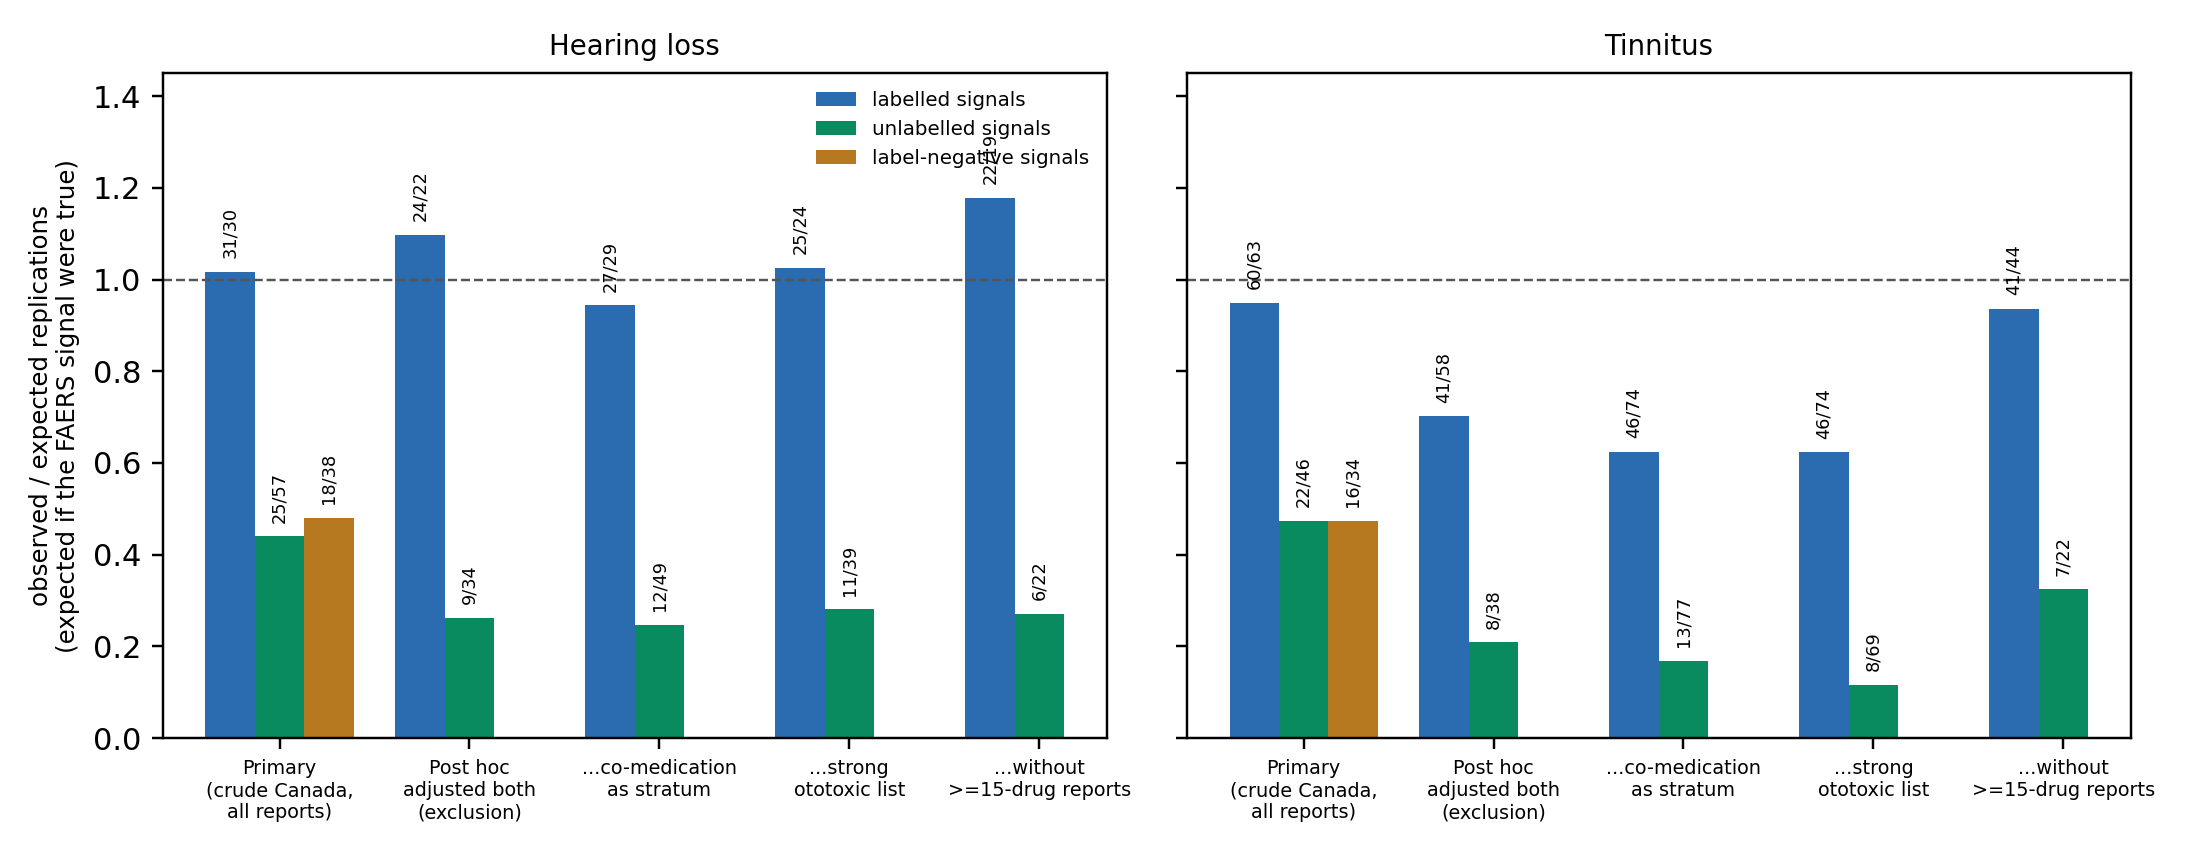
\includegraphics[width=\textwidth]{../figures/replication.png}
\caption{Power-calibrated replication in Canada Vigilance: observed replications divided by those expected if each FAERS
adjusted estimate were true (labels give observed/expected counts). Primary: pre-specified signals, Canada crude estimates,
all reports. Post hoc: both databases adjusted, Canada without solicited reports, four ways of handling co-medication.
A ratio near 1 means signals replicate as their FAERS strength predicts.}
\label{fig:repl}
\end{figure}

\begin{figure}[t]
\centering
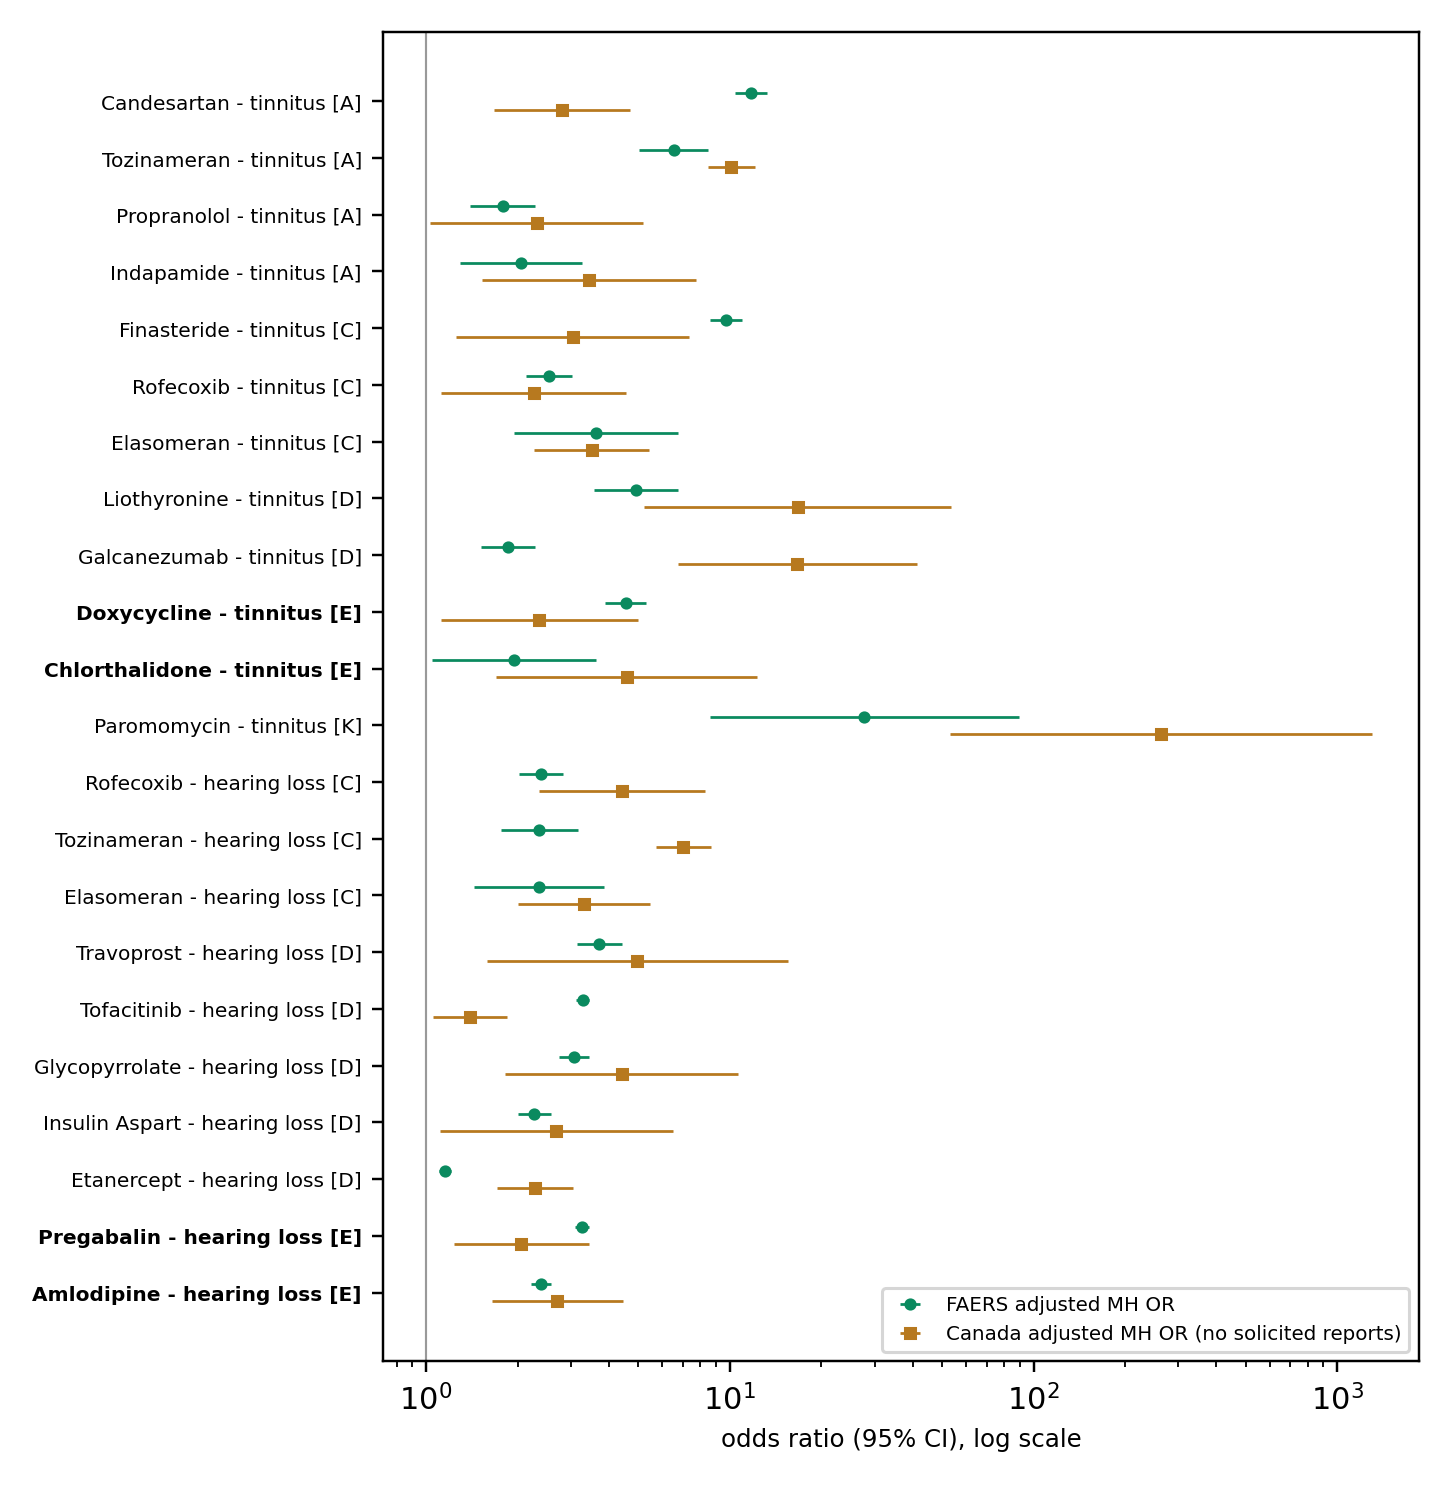
\includegraphics[width=0.85\textwidth]{../figures/candidates.png}
\caption{Robust signals absent from all US labels: FAERS and Canada Vigilance adjusted estimates, with case-review category
(A report cluster; C stimulated reporting; D indication; K established class; E none, bold).}
\label{fig:cand}
\end{figure}


\section{Discussion}
Three findings matter for anyone screening spontaneous reports for ototoxicity. First, adjusting for indication, ototoxic
co-medication, lawyer reports and demographics changed a substantial part of the hearing-loss signal list
(63 of 300 crude signals lost, 73 gained) but did not
improve agreement with labels. Second, replication in an independent national database behaved as a validation test should
for labelled hearing-loss associations---they replicated about as often as their strength predicted---whereas unlabelled
signals replicated less than half as often, a contrast that held within strata of consumer reporting and whose pooled
Canadian estimate (attenuated, not absent) was close to that of signals for drugs whose labels are silent on hearing. Third,
replication is not a clean validator on its own: solicited patient-support-programme reports and report clusters produced
``replications'' for drugs with no known association, and co-medication bias can replicate when crude estimates are compared.
For regulators and signal-management teams, the practical consequence is that replication in a second database does not
strengthen a signal unless reporting artefacts are explicitly addressed.
After adjusted replication, a review of report provenance and an active-comparator check, 7 of 22 robust unlabelled
signals remained (2 to 9 under alternative post-hoc choices and assessors). For tinnitus the same pattern held,
but labelled signals also replicated less fully once both databases were adjusted, so the evidence there is weaker.

These results qualify the previous all-drug screens \cite{li2024,wu2025,liu2025} rather than contradict them. Their
labelled signals largely held; their unlabelled signals mostly did not, and several of the strongest are consistent with how
reports were collected rather than with pharmacology. Tafamidis and sacubitril/valsartan are examples: hundreds to thousands
of FAERS hearing-loss reports, mostly from US consumers and consistent with manufacturer programmes, and none in Canada. The same mechanism
produced spurious Canadian ``replications'' for biologics. Solicited reports are known to distort disproportionality
\cite{psp_solicited}, and their share differs between databases, so report provenance can manufacture both a signal and its
replication.

In this study three steps did most of the work: comparing \emph{adjusted} estimates in both databases;
profiling each case series for concentration---solicited or consumer reports, a single country or year, very drug-dense
reports; and comparing the drug with others used for the same indication. The power-calibrated comparison is simple and avoids
the outcome-dependent testability of rules based on observed counts; it remains sensitive to overdispersion, and empirical
calibration against negative controls \cite{schuemie2014} or regression-based adjustment for co-reported drugs
\cite{caster2010} would be natural extensions. We suggest that screens for hearing outcomes report these provenance
indicators for every signal, in line with the case-by-case item of READUS-PV \cite{readuspv,readuspv_ee}.

The remaining candidates are hypotheses. Pregabalin, an $\alpha_2\delta$ ligand, had 1{,}703
FAERS hearing-loss reports (adjusted OR
3.25 (3.09--3.43))
that replicated in Canada and persisted against other drugs for pain and neuropathy; a case of reversible, dose-related hearing
loss has been described \cite{pregabalin_case}, but age and diabetes confound \cite{diabetes_hearing}, and its labels list
tinnitus and hyperacusis. For amlodipine, hypertension is associated with hearing loss \cite{htn_hearing}, yet the signal
persisted against other antihypertensives, while a large cohort found a \emph{lower} risk of sensorineural hearing loss with
calcium-channel blockers \cite{ccb_cohort}, which argues against a causal effect. Tofacitinib, travoprost and glycopyrrolate
persisted within rheumatoid arthritis, glaucoma and COPD, diseases themselves linked to hearing loss
\cite{ra_hearing,glaucoma_hearing,copd_hearing}, so residual confounding by disease severity remains possible. Doxycycline
can cause intracranial hypertension, of which pulsatile tinnitus is a symptom \cite{doxy_iih}, although few cases reported
it. None of these should change practice without studies that have exposure data.

\paragraph{Limitations.} Spontaneous reports lack exposure denominators, and disproportionality measures reporting, not risk
or incidence. The label reference set is imperfect: labels are partly informed by spontaneous reports, list rare events
without causal assessment, and route-specific labels (for example topical gentamicin) blur ingredient-level status; we used it
only to compare methods. Excluding reports with an ototoxic co-medication conditions on a variable that reporters may add
after observing the event, which pushed some label-positive drugs below 1; stratifying instead removed that artefact but left
residual co-medication bias, and both gave the same replication contrast. Indications are often missing; unreported
co-treatment (for example aminoglycosides in mycobacterial disease) remains; content deduplication was not applied to Canada
Vigilance and cannot catch near-duplicate series, which the report-cluster indicator only partly addresses; and combination
products contribute to each ingredient (valsartan inherits sacubitril/valsartan reports). Canadian reports were removed from
FAERS by occurrence country, or reporter country when missing. The Canada Vigilance documentation does not state that the
extract is domestic; restricting it to reports sent directly to Health Canada gave similar results
(39/72 (54\%) of adjusted signals replicated, background
12/58 (21\%)). About 8{,}100 ingredients were screened without
multiplicity correction; the replication and calibration analyses, rather than individual $p$-values, carry the conclusions,
and the calibration's expected counts depend on Poisson assumptions that the background shows to be optimistic. Corrections
made after the first results (ingredient synonyms, comparator handling for listed drugs, label sections) changed the primary
numbers slightly; they are listed in the protocol file. The solicited-report exclusion, the extended indication filter,
adjusted-to-adjusted and calibrated replication, the co-medication variants, the active-comparator check and the case-level
review were added after the primary results were seen, partly in response to internal review, and are labelled post hoc. The
case-level review was applied by the author and by an AI assessor that used the same profiles and search tools, not by
independent clinicians; the two assessments are therefore not fully independent, and the agreement statistic should be read
in that light. Within-indication comparisons can be affected by channelling (for example tofacitinib as a second-line drug).
FAERS report-source codes that would identify solicited reports directly were not used.

\paragraph{Conclusions.} In FAERS, most drug--hearing-loss signals that are not already on a label do not survive adjusted
replication in Canada Vigilance and a review of report provenance; disproportionality analysis remains a
hypothesis-generating tool. Replication in a second spontaneous-reporting database is informative only when both estimates are
adjusted and solicited reports and report clusters are handled explicitly. The few remaining candidates, with pregabalin the
strongest, are hypotheses that merit study with exposure-based designs, not established adverse effects.

\section*{Statements and declarations}
\textbf{Funding:} no funding was received for this study.
\textbf{Competing interests:} until October 2026 the author was employed as a software engineer at Suno, a company that develops practice-management software for hearing clinics; the company had no role in the design, analysis or reporting of this study, and the author has no financial relationship with manufacturers of the drugs studied.
\textbf{Ethics approval:} not applicable; the study used public, de-identified data.
\textbf{Consent to participate and for publication:} not applicable.
\textbf{Data availability:} FAERS and Canada Vigilance data are publicly available from the FDA and Health Canada; result
tables are in the repository below.
\textbf{Code availability:} code, protocol (\texttt{PROTOCOL.md}, with commit history) and results: https://github.com/olegtropinin/faers-ototoxicity, archived at Zenodo,
\href{https://doi.org/10.5281/zenodo.23659658}{doi:10.5281/zenodo.23659658}.
\textbf{Author contributions:} OT conceived and designed the study, directed and checked the analysis, and wrote and approved
the manuscript.

\bibliographystyle{unsrtnat}
\bibliography{refs}
\end{document}
